\documentclass[12pt,conference]{IEEEtran}
\usepackage[cmex10]{amsmath}
\usepackage{hyperref}
\usepackage{graphicx}
\usepackage{listings}
\usepackage{color}
\usepackage{bbm}

\definecolor{mygreen}{rgb}{0,0.6,0}
\definecolor{mygray}{rgb}{0.5,0.5,0.5}
\definecolor{mymauve}{rgb}{0.58,0,0.82}

\lstset{ 
  backgroundcolor=\color{white},   % choose the background color; you must add \usepackage{color} or \usepackage{xcolor}; should come as last argument
  basicstyle=\footnotesize,        % the size of the fonts that are used for the code
  breakatwhitespace=false,         % sets if automatic breaks should only happen at whitespace
  breaklines=true,                 % sets automatic line breaking
  captionpos=b,                    % sets the caption-position to bottom
  commentstyle=\color{mygreen},    % comment style
  deletekeywords={...},            % if you want to delete keywords from the given language
  escapeinside={\%*}{*)},          % if you want to add LaTeX within your code
  extendedchars=true,              % lets you use non-ASCII characters; for 8-bits encodings only, does not work with UTF-8
  firstnumber=1,                % start line enumeration with line 1000
  frame=single,	                   % adds a frame around the code
  keepspaces=true,                 % keeps spaces in text, useful for keeping indentation of code (possibly needs columns=flexible)
  keywordstyle=\color{blue},       % keyword style
  language=R,                 % the language of the code
  morekeywords={*,...},            % if you want to add more keywords to the set
  numbers=left,                    % where to put the line-numbers; possible values are (none, left, right)
  numbersep=5pt,                   % how far the line-numbers are from the code
  numberstyle=\tiny\color{mygray}, % the style that is used for the line-numbers
  rulecolor=\color{black},         % if not set, the frame-color may be changed on line-breaks within not-black text (e.g. comments (green here))
  showspaces=false,                % show spaces everywhere adding particular underscores; it overrides 'showstringspaces'
  showstringspaces=false,          % underline spaces within strings only
  showtabs=false,                  % show tabs within strings adding particular underscores
  stepnumber=2,                    % the step between two line-numbers. If it's 1, each line will be numbered
  stringstyle=\color{mymauve},     % string literal style
  tabsize=2,	                   % sets default tabsize to 2 spaces
  title=\lstname                   % show the filename of files included with \lstinputlisting; also try caption instead of title
}
\hyphenation{op-tical net-works semi-conduc-tor}
\pagenumbering{gobble}

\begin{document}
\title{Non-Parametric Genomic Fourier Power Spectra Filter Designs}
\author{Micah~Thornton,~\IEEEmembership{Student Member,~IEEE,}
        and~Monnie~McGee,~\IEEEmembership{Member,~IEEE,}% 
\IEEEcompsocitemizethanks{\IEEEcompsocthanksitem M. Thornton is with the Lyda Hill Department
of Bioinformatics, University of Texas Southwestern, Dallas,
TX, 75390.\protect\\
E-mail: \url{mailto:mathornton@smu.edu}
\IEEEcompsocthanksitem M. McGee is with the Department of Statistical Science at Southern Methodist University, Dallas, TX, 75206.\protect\\
E-mail: \url{mailto:mmcgee@smu.edu}}% 
\thanks{Manuscript received June 10, 2021}}%; revised July ??, 2021}}

\markboth{Eighth Biomedical Circuits and Systems Conference,~October~2021}%
{Thornton \MakeLowercase{\textit{et al.}}: Fourier Power Spectra No-Lag Matched Filters for Genomic Sequence Differentiation}
\IEEEtitleabstractindextext{%
\begin{abstract}
The comparison of genomic sequences is a important undertaking, the granularity with which the sequences are to be compared varies by application.  In this work we describe three procedures that 
can be applied to genomic power spectra of any lengths to reduce their breadth while maintaining the relative 
distances which they provide.  Specifically we present: \textit{minimal variance filtering}, where the 
subsets of coefficients with the highest variance across a sample are selected, \textit{Automated filter 
learning}, where a set of linear combinational filters are learned automatically by a 1-D deep convolutional neural network attempting to classify sequences on region of origin, and \textit{Maximal Variance Principal Components Filters} that provide a set of filters in the Principal component loadings determined among the highest variance elements of the PS for a sample.  We provide a comparison of these approaches by examining their conservation of distances produced by 
the entire PS, and conclude with remarks about the benefits and drawbacks of each method while providing future avenues of pursuit for this research. 
\end{abstract}
\begin{IEEEkeywords}
Genomic Signal Analysis,  Genomic Power Spectra Filtering,  Genetic sequence analysis, Genomic Power Spectra Convolutional Networks, Biomolecular sequence Frequency filtering, Virus Genomic Fourier Power Spectra Filtering. 
\end{IEEEkeywords}}

\maketitle

\IEEEdisplaynontitleabstractindextext

\IEEEpeerreviewmaketitle

\vspace{- 1 em}
\section{Introduction}
\label{sec:int}

\IEEEPARstart{G}{enomic} sequences are, in essence, radix four discrete-index signals, 
and contain essential information required to instantiate and replicate organisms, or non-living matter 
such as viruses and proteins.
These sequences are radix-four as a repetitive series of four base nucleotides: adenine, cytosine, guanine, 
and thymine, in Deoxyribonucleic Acid (DNA) with thymine is replaced by uracil in Ribonucleic Acids 
(RNA) constitute the information conveyed by the signals. 
Notably this characterization considers the base form of the genomic sequences as a four-valued signal, 
some prior works have considered using the hydrophobicity of the translated amino acids in conjunction 
with spectral methods for the identification of attributes of a sequence. \cite{Shu17} 
Other works have examined epigenetic marker profiles using signal detection theory \cite{San19}.
in this work we consider utilization of subsets of characteristic genomic Fourier power spectra which are
produced by a few different kinds of filtering techniques for examining distances between SARS-CoV-2 virus genomes. 
This work treats genomic sequences as signals, and defines procedures for reducing the Mixed-Radix \cite{Sin69} Fourier Power Spectra (PS) of these sequences such that Euclidean distances amongst them are preserved. 
\vspace{-0.5 em}
\section{Prior Works}
\label{sec:pw}
The concept of taking Discrete-Time Fourier Transforms (here ``time'' refers to loci along a genomic signal) 
of genomic signals dates back to the early 1990`s.  Anastassiou provides a summary of these and other
genomic signal processing techniques \cite{Ana01}.
More recently, genomic signals have been investigated from the perspective of 
Information and Fluctuation theory \cite{Dem14}.  
Yin et al. were the first to suggest the use of Fourier coefficients, and the resultant power spectra as 
numerical summaries for distance calculations and subsequent automated phylogeny construction with 
genomic sequences \cite{yin20, yin14, yin15,pei19,Hoa15}.
In these works the power spectra of the coefficients were subject to an even stretching (scaling) procedure 
where power spectra of shorter sequences were extended such that all sequences were of the same length
\vspace{-0.5 em} 
\subsection{Encoding \& Transforming Genomic Sequences}
Genomic/proteomic signals when digitized are usually stored in ASCII text encoded files known as FASTA/Q 
files.  Initially this acronym stood for Fast-All, referring to the capability to store any alphabet based 
sequence, for biomolecular sequences these refered to mostly genetic and proteomic sequences \cite{Lip85}.  
Prior to their storage in FASTA files, NT sequences are presented in the organic materials within which they reside, an enormously dense and resilient storage system the likes of which our engineers have not been able to reproduce. 
Once the material has been analyzed using one of many different sequencing technologies (for a nice review of modern sequencing techniques see Metzker \cite{Met10} or Slatko \cite{Sla18}) it is generally stored either directly in FASTA/Q or sometimes intermediary files (such as intensity images for micro-array data). 
Generally the genomic sequence data once captured is processed using one of a set of bioinformatic procedures. 
Usually assembly or alignment is the desired goal of researchers working with genetic data from the 
earliest stages, and one of the many bioinformatic tools designed for the purpose.  
Some popular examples of aligners include: HISAT, \cite{kim15} HISAT2\cite{Kim19}, bowtie2 \cite{lan12}, and BWA \cite{li09}  (for general DNA sequencing) or aligners like HISAT3N \cite{Zha20} (for sequencing Bisulfite-treated reads).
Following this, the sequences (usually stored in FASTA/Q again after intermediate processing through SAM/BAM formats)
Next the user will generally determine whether they wish for the sequence to be encoded using four-vectors or two-vectors \cite{Vos92}. 
The mapping into four vectors is displayed below in Equation \ref{eqn:fvec}, and one of the possible two-vector encodings for reference is displayed in Equation \ref{eqn:tvec}. 

\noindent {\small
\begin{align}
\begin{split}
\label{eqn:fvec}
V_4[\cdot] &\equiv \{A,C,G,T/U\} \mapsto \\
& \{ [1,0,0,0]^T,[0,1,0,0]^T,[0,0,1,0]^T,[0,0,0,1]^T\}
\end{split}
\end{align}
}
\vspace{-1 em}

\noindent {\small
\begin{align}
\begin{split}
\hspace{-8 em}
\label{eqn:tvec}
V_{2AT}[\cdot] &\equiv\{A,C,G,T/U\} \mapsto \\
& \{ [0,-1]^T,[-1,0]^T,[1,0]^T,[0,1]^T\}
\end{split}
\end{align}
}
\vspace{-0.5 em}

Once one of these transforms is applied to the sequences in order to produce a series of numerical vectors, 
the PS as described by Singleton in 1969 \cite{Sin69} is applied to either the 
four signals (when using $V_4$)  or two signals (when using, for instance, $V_{2AT}$) and the results 
are averaged together by position, providing a single PS of the same length as the initial signal. 

\vspace{-0.5 em}
\subsection{Evenly Scaling Power Spectra} 
To perform direct comparisons of one sequence to another, the ensemble which is being compared
may have their power spectra stretched out to be of the same length as that of the maximal length in 
the sequence.  The procedure by which this is done is described initially by Yin and Yau \cite{yin15} in 
their work describing distances computed using the distance between DFT PS.  The procedure 
scans through the shorter sequence and takes either a single PS coefficient, or a pair of coefficients to 
produce a signal of the same length as the longer.  The formula used is expressed in Equation \ref{eq:evscal}. 


Formally, let $A_n$ denote the original power spectrum of length $n$, and $A_m$ denote the extended power spectrum of length $m$, where $m > n$. The even scaling operation from $A_n$ to $A_m$ is given by
\vspace{-0.5 em}
{\small
\begin{align}
\begin{split}
&A_m(k)=\\
&\begin{cases} A_n(Q) & \mbox{if } Q\in Z^+\\
 A_n(R) + (Q-R)(A_n(R+1)-A_n(R)) & \mbox{if } Q  \notin Z^+
\end{cases}
\label{eq:evscal}
\end{split}
\end{align}
}

\vspace{-0.5 em}
\noindent where $Q = \frac{kn}{m}$ and $R = \lfloor \frac{kn}{m} \rfloor$ \cite{yin15}. This even scaling algorithm is extensible to signal length differences of up to one half the size of the smaller signal without providing substantive loss in terms of information content.

\vspace{-1 em}
\begin{figure}[h!]
\caption{Genomic Signal Flow Diagram for Mixed-Radix Power Spectra Calculation} 
\label{fig:fftflow} 
\begin{center} 
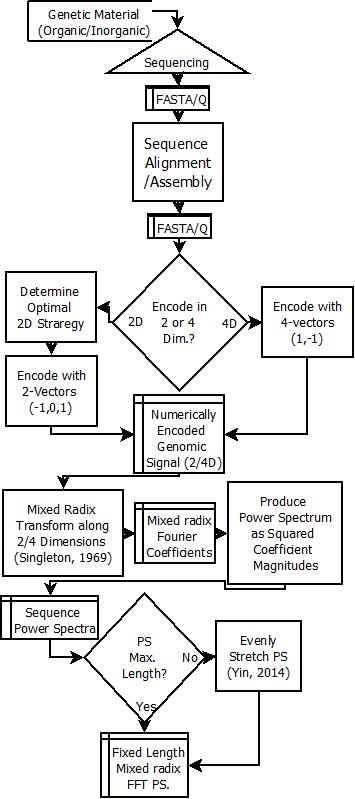
\includegraphics[scale=0.45]{Images/Files/GenomicFFTSignalFlow.png}
\end{center} 
\end{figure} 


A signal flow diagram describing the entire flow of information from the genetic material the genomic 
signal was extracted from all the way down to the produce power spectra ensemble is shown in Figure 
\ref{fig:fftflow}.  The \textit{evenly scaled} PS are the numerical summaries of the sequences to which 
the subsequent filtering and characteristic learning procedures described in the methods section are applied.


\section{Methods \& Design}
\label{sec:meth}

The approaches discussed here seek to determine appropriate subsets of the PS 
which may be used to appropriately numerically summarize genomic signals such as DNA and RNA. 
These procedures seek to reduce the extent of the PS analyzed while maintaining the
relative ordering of distances among the pairs of sequences analyzed.  
In this work, three different approaches to filtering the PS are suggested, and there relative utilities are 
assessed, by using Pearson's Correlation coefficient to measure the similarity between the Euclidean 
distances produced when using the full unfiltered PS, and those produced when using the filtered PS. 
Each of the approaches suggested are applicable only after a substantive base data supply has been 
collected. 
This means that for new genomic signals which are collected, the same filters may be applied to their 
PS, however if the filters themselves were to be reconstructed with the data set that includes the newly 
gathered signals, than they may not be identical to those that are produced by a subset of the data. 

\subsection{Minimal Variance Filtering} 

The first approach discussed is based on a single value, the percentage of PS coefficients to filter. 
After the PS have been computed for a sample of data a researcher wishes to compare, the variance of either the entire 
sample, or some representative subsample at each position along the PS is computed, next the user supplied filtering 
parameter $q$, the fraction of the coefficients by which to reduce the original PS, is used to determine which variance should be the cutoff in the data.  

\vspace{-1 em}
\begin{align} 
\label{eq:var}
\begin{split}
v_j =& \frac{\sum_{i=1}^N\left(S_{ij}-\frac{\sum_{i=1}^N(S_{ij})}{N}\right)^2 }{N-1} \\
\eta^* =& \left\{ v_j \Bigg\vert \sum_{k=1}^m \mathbbm{1}\left( v_j \leq v_k \right) = \lfloor m\cdot q\rfloor \right\}\\
S^*_{il} =& \left\{ S_{ij} \Bigg\vert v_j \geq \eta^* \right\}
\end{split}
\end{align}

\vspace{-0.5 em} 
Equation \ref{eq:var} shows how a variance filtering approach can be applied to 
a genomic PS coefficient $j = 1,2,\dots m$ for sample $i = 1,2,\dots,N$, $S_{ij}$ to produce  the filtered PS $S_{il}$ for $l = 1,2,\dots,\lfloor m \cdot q \rfloor$. 
In other words, the filtered PS $S_{il}$ are produced by selecting only those PS coefficients from the unfiltered PS that have the largest across sample variances. 
In the results section we will see how this approach to filtering the PS changes the 
distances that are calculated amongst the elements of the sample.  This filtering process may be considered as semi-analagous to that of a \textit{matched filter} from 
traditional signals processing.  
As a matched filter seeks to exploit a template, so too does the minimal variance filtering technique, in that once 
a threshold determination is made from the composite variances of the coefficients then each of the PS are
matched to it  by selection only if the PS coefficients had a higher variance.  
The variance filtering technique does not  inspect the composite variances at various lagged values though, and hence is only similar to the lag-zero matched filter. 

\subsection{Automated Filter Learning} 

A second approach to filtering is less \textit{hands-on}, and provides not a binary filter such as the \textit{minimal variance filtering} technique,  but a set of filters 
that are unique linear combinations of the entire Genomic PS are determined 
automatically by a Convolutional Neural Network (CNN).  A schematic of the 
Machine Learning (ML) approach is shown in Figure \ref{fig:mlschem} .

\begin{figure}[h!]
\centering
\caption{Schematic of Machine Learning approach for automatic filter learning \label{fig:mlschem} }
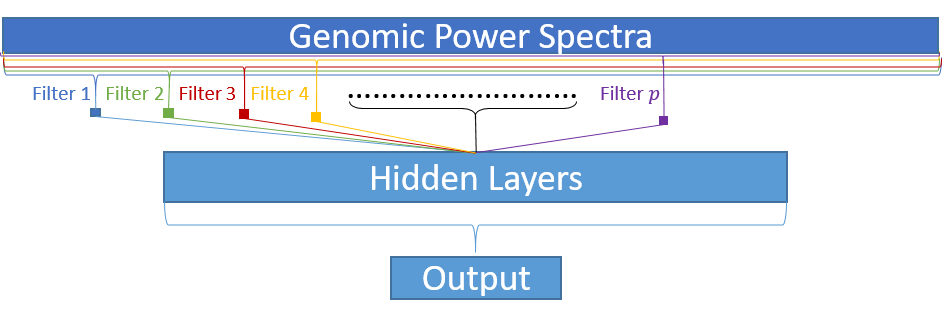
\includegraphics[scale=0.5]{Images/Files/afl.png}
\end{figure}

As with the previous approach, the size of the filtered PS can be fixed programatically by the researcher,
here however, the resultant set of filtered PS coefficients actually consist of linear combinations of 
all of the unfiltered PS coefficients.  This procedure is dependent on having some sort of supervised 
labels for each of the sequences used to construct the filters.  These labels will help to determine the 
kinds of filters constructed, so the aspects of the original PS that help differentiate the elements of the 
sample on the chosen labels will be extracted by the filters learned.  Here the convolutional network 
layer is applied to the entire length of the PS, we leave it to future work to examine shorter filters which
slide across the length of the PS.  The length of the filtered PS in this case can be selected as $p$, which
is the number of different filters to be learned by the CNN.  Note that the filters learned also depends 
on the Hidden layers between the output and the convolutional layer.  In the results section we will 
look at a specific architecture that learns filters by attempting to classify the region of submission of 
the sequences. 

\subsection{Maximal Variance Principal Components}

As an extension of the \textit{minimal variance filtering} and hybridized approach, providing linear combinational filters 
in the same style as those automatically learned in the CNN approach we may consider applying PCA 
to the highest variance coefficients in the sample from which the filters are constructed. 
Assuming that the number of samples to construct the filter from $N$ is shorter than the PS 
length $m$, this technique will select the $N$ highest variance PS coefficients, and apply PCA to them
in order to produce linear combinations of these PS which maximize the variance, to serve as filters. 
In this case, the user may select the length of the filtered PS by selecting the first $k$ principal 
components. 
Note that if it is the case that $N \geq m$ then all of the unfiltered PS coefficients may be supplied to 
the PCA procedure. 

\section{Results} 
\label{sec:res}

The procedures described in Section \ref{sec:meth} are applied to a sample of viral genomes
submitted by various labs during the 2020 SARS-CoV-2 pandemic curated by the GISAID Initiative \cite{gisaid}. 

\subsection{Minimal Variance Filtering} 

Firstly, the minimal variance filtering approach is applied to the set of PS for the virus genomes. 

\begin{figure}[h!] 
\caption{(a) Scatter plot of PS coefficient variances for 1,397 SARS-CoV-2 Genomes, (b) Histogram of PS coefficient variances, (c) Survival Plot of Coefficients by Variance, (d) Pearson's $\rho$ between filtered PS distances and full PS distances. \label{fig:coeffvar}} 
\centering
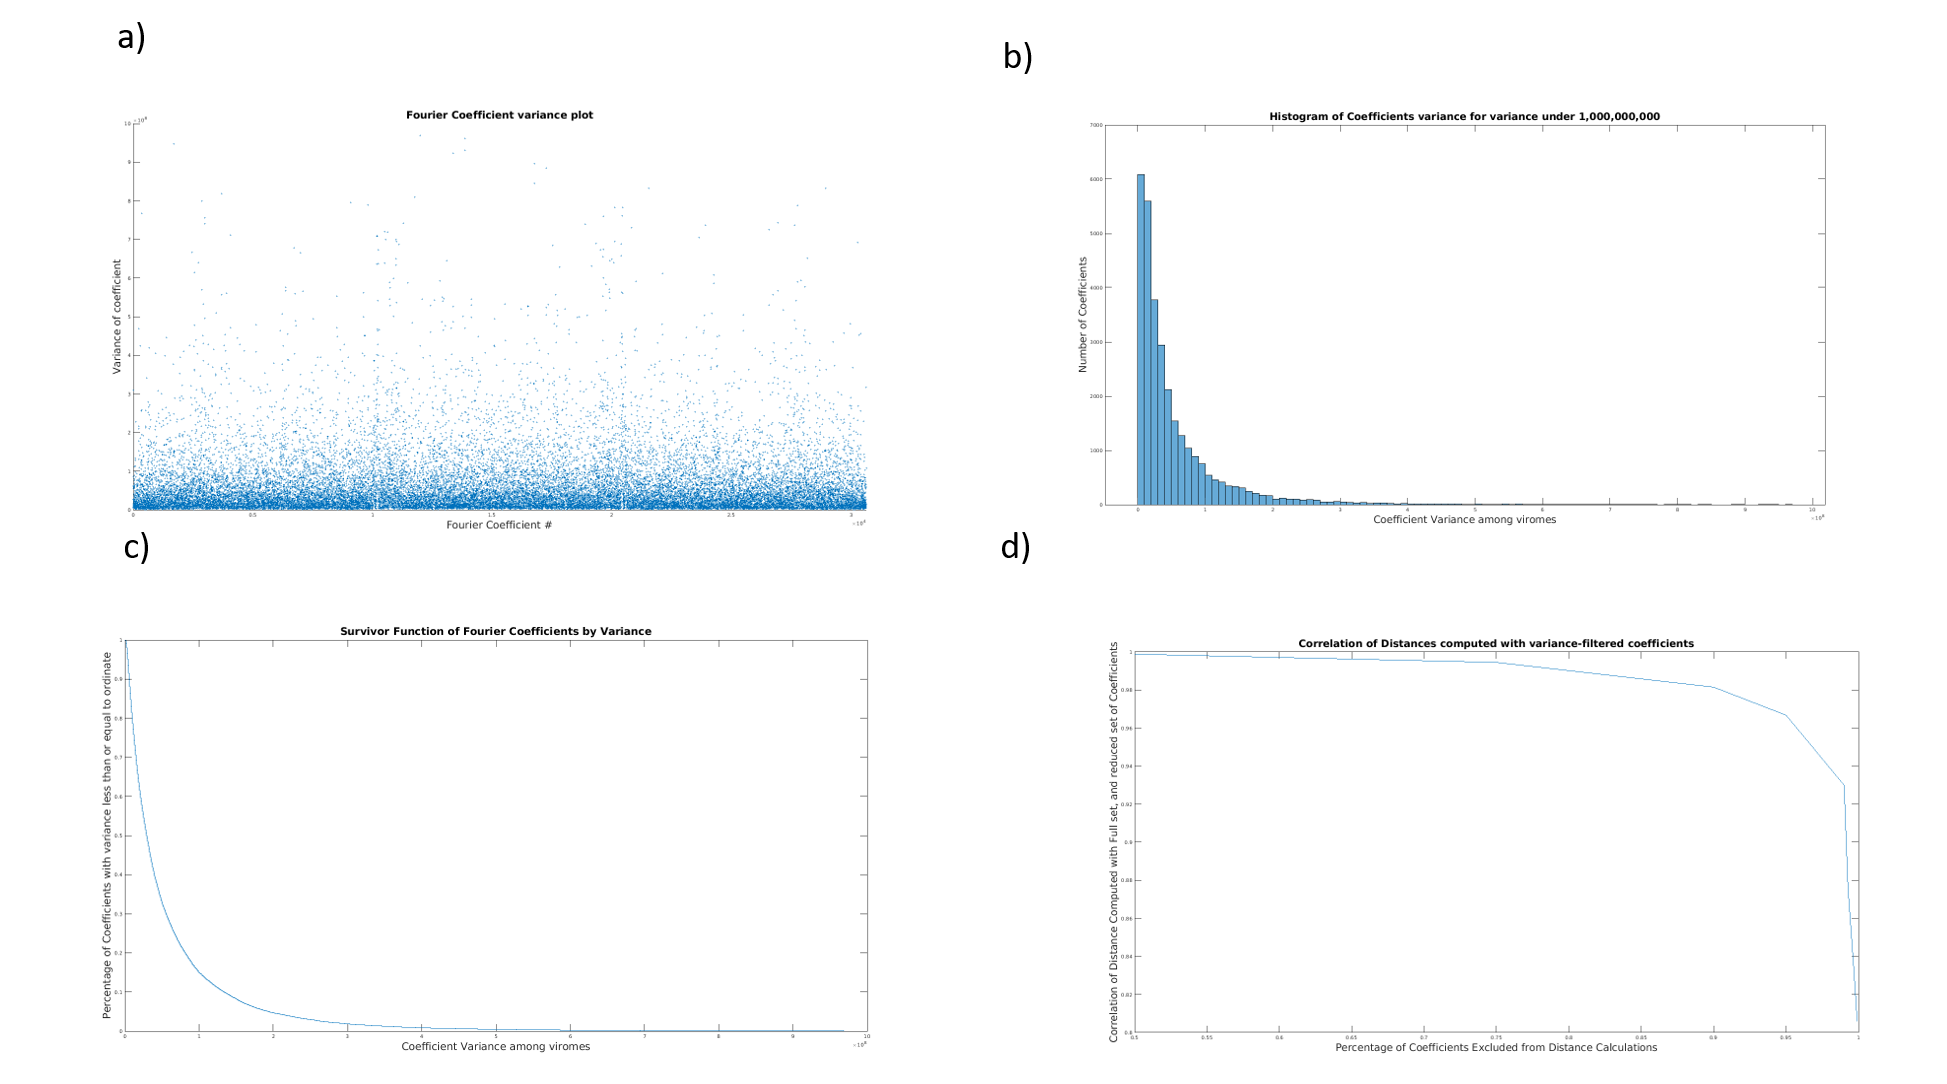
\includegraphics[scale=0.27]{Images/Files/VarianceFiltCombined.png}
\end{figure}


Figure \ref{fig:coeffvar} (a) displays a scatter plot of the variances of each generated set of PS Coefficients for the 1,397 viral genomes included in the study.  On this plot, a filter applied to the 
coefficients may be selected by examining only the coefficients that have a larger variance than some threshold value, graphically a horizontal line. 
A histogram of some of the selected coefficients is displayed in Figure \ref{fig:coeffvar} (b), where 
a filter may graphically be considered as a vertical line, beyond which the area
highlighted is the amount of coefficients that are included in the distance calculation phase.  
Figure \ref{fig:coeffvar} (c) displays the survival curve of coefficients by their variance, that is, the
percentage of coefficients with variance greater than or equal to the ordinate is displayed as the 
abscissa. Figure \ref{fig:coeffvar} (d) displays the correlation of distances when using the full PS, and the filtered PS with the percentage of coefficients filtered on the x-axis. 


\subsection{Automated Filter Learning}
\begin{figure}[h!]
\centering
\caption{(a) Image produced from scaled Unfiltered PS for all 1,397 Viral genomes (30,563 coefficients) (b) CNN Weights learned for 30,563 PS, for 128 Filters (c) Each of the 1,397 full PS (30,563) filtered into 128 values (d) The 20 highest variances filtered PS among the 128.  \label{fig:CNN128Filts}}
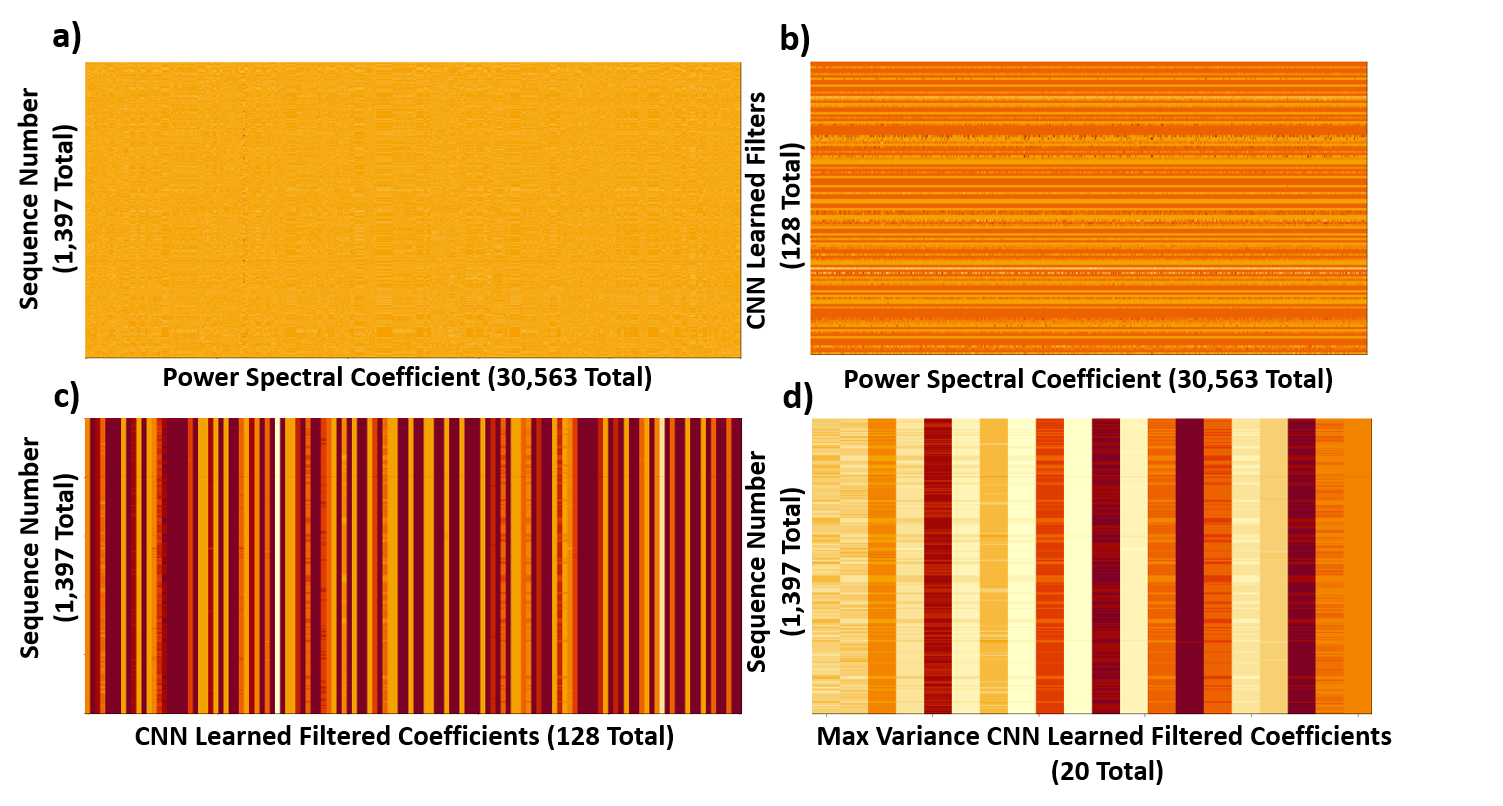
\includegraphics[scale=0.35]{Images/Files/CNNFilters.png}
\end{figure}

A CNN for classifying the GISAID August SARS-CoV-2 PS on their region of submission for eight general regions extracted from the headers was implemented and trained using the `keras' package \cite{kerR21}, 
which extends an interface to the `keras' framework in R.

The initial deep network trained 128 filters, on the entire data set over 20 epochs, with a batch size of 140. 
The results of these 128 filters are graphically represented in Figure \ref{fig:CNN128Filts}.
For the comparison section, the CNN is retrained with different numbers of filters in order to provide a 
valid filtered PS set for comparison to the other two methods. 
\subsection{Maximal Variance Principal Components}

The last of the filtering approaches discussed allows for slightly less customization in terms of the filtered PS 
length. 
Here for instance, there are a total of 1,397 sequences, which is less than the length of the unfiltered PS (30,563). 
This method explicitly seeks to determine the overall linear combination which maximizes the variation across the entire 
set of sequences. 
%\begin{figure}[h!] 
%\centering
%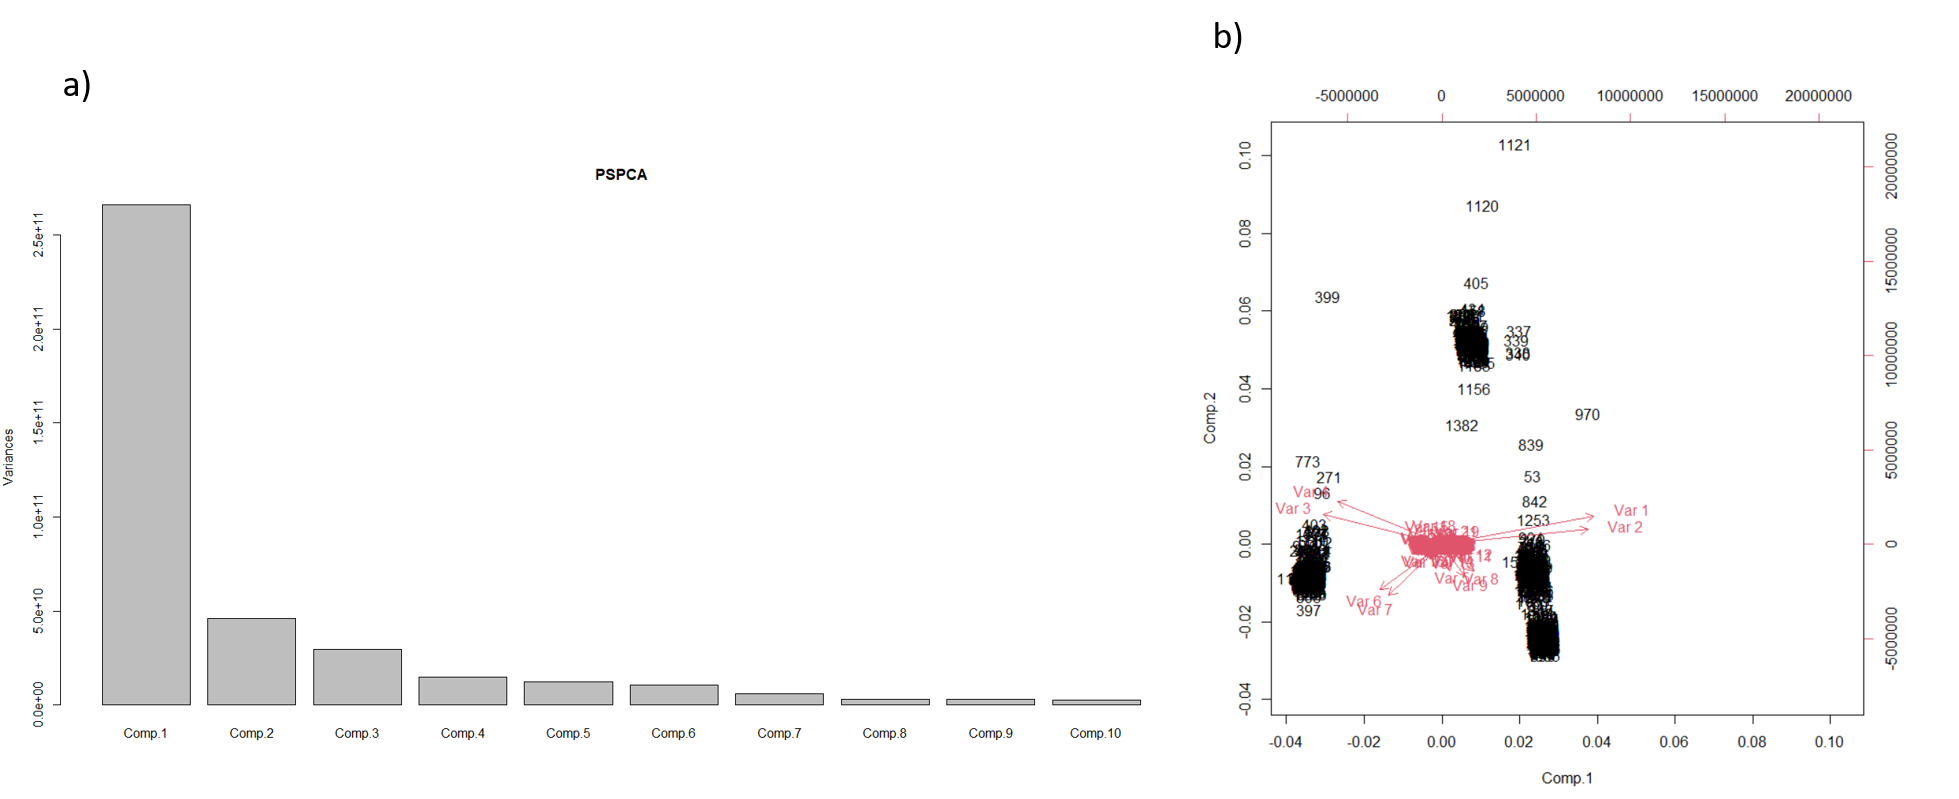
\includegraphics[scale=0.26]{Images/Files/PCAResults.png}
%\end{figure} 

\subsection{Method Comparison} 

\begin{figure}[h!]
\caption{Filtering Methods Comparisons, by Correlation to Full PS Distances \label{fig:filtcomp}}
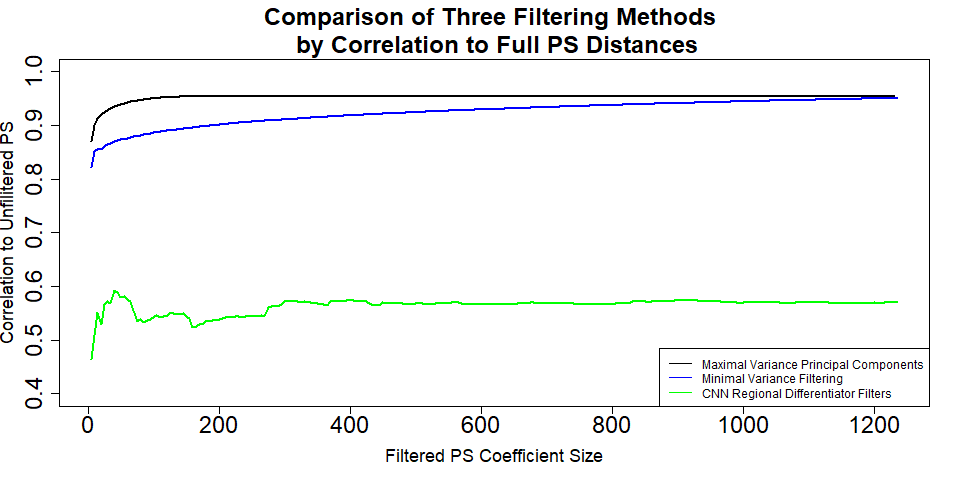
\includegraphics[scale=0.18]{Images/Files/PSFiltMethods.PNG}
\end{figure}

When comparing the three filtering methods discussed in this work on the SARS-CoV-2 data set, the Principal Components procedure performs 
the best, when filtering the original PS down to around 1,235 coefficients, however as noted before, one of the primary 
drawbacks of the PCA procedure is that it can only be used to filter the original PS to the number of sequences used to 
construct the features, therefore it is likely that the distances produced by the minimal variance filtering for more coefficients than are available in the largest subset produced by the PCA will have greater correlation than achievable with 
the PCA approach. 


Perhaps one of the most surprising aspects of Figure \ref{fig:filtcomp} is the low correlation from the CNN trained 
filters.  
Likely these filters extract information more relevant to differentiating the region of submission, than correlating to the 
full PS distances, which explains this result. 
\section{Conclusions}

In this work we show that a comparison of a subset of the initial PS produced for comparing genomic 
sequences can be used to determine distances that are highly correlated with the entire set. 
This work is beneficial as it allows for a smaller set of the PS than the full length PS to represent genomic signals, and 
determine distances. 

\label{sec:conc}

\subsection{Directions and Future Works} 

Using pairwise ratios and differences of specific parts of the PS we will be able to use statistical hypothesis testing theory in order to directly derive expressions for the parameters of the F and Variance-Gamma distributions respectively to determine the probability that two sequences came from the same 
source.  A distributional test for the maximal PS coefficients based on the ratio/difference of the asymptotic 
distribution in the domain of attraction of the Gumbel distribution (as proven by McGee and Ensor \cite{mcg98}) could also be developed. 
As previously stated, these filtering techniques may be extended in a few directions, the automatic learning with the CNN 
can be extended to examine truly convolutional filters of shorter length than the full signal. 


\appendices
\vspace{-1 em}
\section*{Acknowledgment}
{\small
The work in this paper would not have been possible without the support of the Daehwan Kim Lab in 
the Lyda Hill Department of Bioinformatics at UTSW.  In the results section the SARS-CoV-2 viral 
genomes captured from the GISAID Initiative \cite{gisaid} reflect the combined efforts of many labs, 
for a complete listing please see \url{https://tinyurl.com/8ptzru7s}.
}

\bibliographystyle{IEEEtrans}
\bibliography{2021BioCASRef}

\section{Acronym Dictionary} 
{\tiny
\begin{itemize} 
\item \textbf{ASCII} - American Standard Code for Information Interchange
\item \textbf{BAM} - Binary Alignment Map. 
\item \textbf{CNN} - Convolutional Neural Network (Typically 1-Dimensional as applied to Genomic PS)
\item \textbf{DFT} - Discrete Time Fourier Transform (Usually Discrete Loci, Mixed-Radix Transform)
\item \textbf{DNA} - Deoxyribonucleic Acids (Genetic Material stored in Eukaryotic Nuclei)
\item \textbf{FASTA/Q} - Fast-All File format (Q - Quality Scores)
\item \textbf{FFT} - Fast Fourier Transform (Usually Mixed Radix)
\item \textbf{GISAID} - Global Initiative on Sharing All Influenza Data (Initiative curating SARS-CoV-2 Genomes)
\item \textbf{ML} - Machine Learning
\item \textbf{NT(s)} - Nucleotide(s) (referring arbitrarily to Adenine, Cytosine, Guanine, and Thymine (or Uracil))
\item \textbf{PCA} - Principal Components Analysis
\item \textbf{PS} - Power Spectra (Usually Mixed-Radix Fourier Power Spectra)
\item \textbf{RNA} - Ribonucelic Acids (Genetic Material transcribed from DNA, existing outside Nuclei)
\item \textbf{SAM} - Sequence Alignment Map (A format usually outputted from aligners which displays the locations of reads along a reference). 
\item \textbf{SARS-CoV-2} - Sudden Acute Respiratory Syndrome Coronavirus 2 (Virus responsible for 2019- Pandemic)
\item \textbf{SMU} - Southern Methodist University (University in Dallas Texas) 
\item \textbf{UTSW} - University of Texas Southwestern (Medical Center \& University in Dallas, Texas)
\end{itemize}
}

\section{Software Repository \& Tutorial Video}
{\small
This software was written using the R-Programming Language (R version 4.1.0 (2021-05-18) -- ``Camp Pontanezen") \cite{r21}.   For the automated filter learning via CNN the `keras' R Interface is utilized \cite{kerR21}.  The Tensorflow R-Package was also used for 
accessing the capabilities extended by the tensor flow \cite{tfR21}.  The Genomic DFT power spectra for the viruses as well as the virus data themselves are contained within an R package we wrote \cite{dftR}, which may be installed from the R-console using the following: 

\begin{lstlisting} 
library(devtools);
install_github('mathornton01/Genomic-DFT-Yin-R'); 
\end{lstlisting} 
\vspace{-2 em}

A short ($\approx$ 3:00) tutorial video showing how to install the software referenced above, and apply 
the techniques to an example data set is available at \url{https://people.smu.edu/mthornton/} 
}
\begin{IEEEbiographynophoto}{Micah Thornton}
Is a fourth year Ph.D. candidate in a joint Southern Methodist University (SMU) and University of Texas Southwestern (UTSW) Biostatistics Program.  Micah holds a Bachelor's of Science (B.S) in Computer Engineering, a B.S. in Statistical Science, and a Master's of Science (M.S) in Computer Engineering from SMU. 
\end{IEEEbiographynophoto}

\begin{IEEEbiographynophoto}{Monnie McGee} 
Is an associate professor in the Department of Statistical Science at SMU. Monnie holds a Bachelor's of Arts (B.A) in Mathematics and English from Austin College, and a Master's of Arts and Doctor of Philosophy in Statistics from Rice University.  

\end{IEEEbiographynophoto}

\end{document}


